\documentclass[a4paper,12pt]{article}

\usepackage{geometry}
\geometry{margin=1cm, lmargin=3cm, bmargin=2cm}

\usepackage[T2A]{fontenc}
\usepackage[utf8]{inputenc}
\usepackage[english,russian]{babel}

\usepackage[nottoc,numbib]{tocbibind} %for adding bibliography to 
                                      %table of content

\usepackage{color}   %May be necessary if you want to color links
\usepackage{hyperref}
\hypersetup{
    colorlinks=true, %set true if you want colored links
    linktoc=all,     %set to all if you want both sections and subsections linked
    linkcolor=black, %choose some color if you want links to stand out
    citecolor=black,
}

\addto\captionsrussian{\renewcommand{\refname}{Источники}}
\setlength{\parindent}{0em}
\setlength{\parskip}{1em}

\usepackage{graphicx}
\graphicspath{ {./../img/} }

\usepackage[font=small,labelfont=bf]{caption}

\usepackage{amsmath}

\usepackage{float}

\begin{document}

\begin{titlepage}
  \centering

  \vspace*{3em}
  
  % Name of the university
  Санкт-Петербургский Государственный Университет \\
  Факультет прикладной математики – процессов управления \\[15em] 

  { \large 
  Работа по курсу \\
  «Методы и средства научной визуализации» \\
  на тему 2.4 «Самоорганизующаяся карта Кохонена»\\[10em]
  } % Title

  \begin{flushright} %author's name
    Работу выполнял \\
    студент 331 группы \\
    Козырев Сергей Александрович \\[10em]
  \end{flushright}

  \today
\end{titlepage}

\newpage
\tableofcontents

\newpage

\section{Введение}

При анализе и прогнозировании социально-экономических явлений исследователь довольно часто сталкивается с многомерностью их описания. Это  происходит при решении задачи сегментирования рынка, построении типологии стран по достаточно большому числу показателей, прогнозирования конъюнктуры рынка отдельных товаров, изучении и прогнозировании экономической депрессии и многих других проблем.\cite{intro1} Всё это можно отнести к задачам кластеризации.

\textbf{Кластеризация} (англ. cluster analysis) — задача группировки множества объектов на подмножества (кластеры) таким образом, чтобы объекты из одного кластера были более похожи друг на друга, чем на объекты из других кластеров по какому-либо критерию. Задача кластеризации относится к классу задач обучения без учителя.\cite{clustering}

Задача кластеризации данных (также называемая таксономией, автоматической классификацией или группировкой объектов) является одной из наиболее важных и сложных задач анализа данных. Кластерный анализ представляет собой раздел статистического анализа данных, объединяющий методы разбиения (группировки) множества наблюдаемых объектов на сравнительно однородные группы, называемые кластерами. Однородность кластеров означает, что объекты, отнесенные к одному кластеру, должны быть близки относительно выбранной метрики. Объекты из разных кластеров должны существенно отличаться. Кластерный анализ является востребованной и успешно развивающейся дисциплиной современной теоретической информатики. Его методы имеют широкий спектр применений практически во всех областях человеческой деятельности, связанных с изучением объектов и процессов: медицине, биологии, химии, маркетингу, психологии, социологии, менеджменту, филологии, археологии и другим.\cite{intro2}

Именно задачу кластеризации решает самоорганизующаяся карта Кохонена, которой посвящена данная работа.

\subsection{История}

Эту нейронную сеть предложил финский профессор Теуво Кохонен в 1980-х годах. Самоорганизующаяся карта Кохонена (SOM) выросла из ранних моделей нейронных сетей, особенно моделей ассоциативной памяти и адаптивного обучения (ср. Кохонен 1984). Новый стимул состоял в том, чтобы объяснить пространственную организацию функций мозга, особенно наблюдаемую в коре больших полушарий. Тем не менее, SOM не была первым шагом в этом направлении: следует упомянуть, по крайней мере, пространственно упорядоченные линейные детекторы фон дер Мальсбурга (1973) и модель нейронного поля Амари (1980).

Первой областью применения SOM было распознавание речи (см. рис. \ref{fig:phonemesom}). В своей абстрактной форме SOM получила широкое распространение в области анализа и исследования данных (Kaski et al. 1998, Oja et al. 2003, Pöllä et al. 2007).\cite{scholarpedia}

\begin{figure}[H]
  \centering
  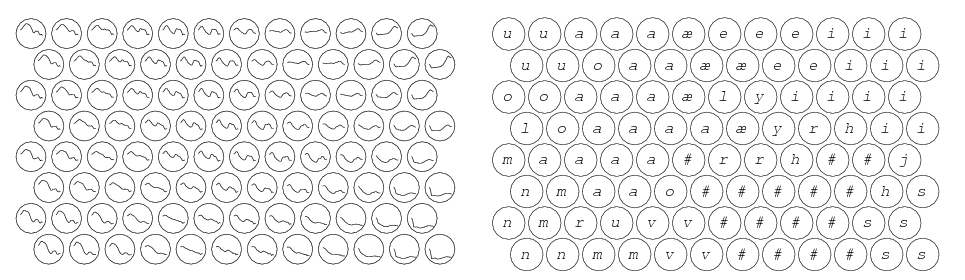
\includegraphics[width=1\textwidth]{Phonemesom.png}
  \caption{Левое изображение: модели акустических спектров финских фонем, организованных на некотором расстоянии.
  Правое изображение: калибровка моделей по фонемным классам. Символ \# обозначает взрывные согласные /k, p, t/.}
  \label{fig:phonemesom}
\end{figure}

\subsection{Задачи, решаемые при помощи карт Кохонена}

Самоорганизующиеся карты могут использоваться для решения таких задач, как моделирование, прогнозирование, поиск закономерностей в больших массивах данных, выявление наборов независимых признаков и сжатие информации.

Наиболее распространенное применение сетей Кохонена - решение задачи классификации без учителя, т.е. кластеризации.

Напомним, что при такой постановке задачи нам дан набор объектов, каждому из которых сопоставлена строка таблицы (вектор значений признаков). Требуется разбить исходное множество на классы, т.е. для каждого объекта найти класс, к которому он принадлежит.

В результате получения новой информации о классах возможна коррекция существующих правил классификации объектов.

Вот два из распространенных применений карт Кохонена: разведочный анализ данных и обнаружение новых явлений.

\textbf{Разведочный анализ данных.} Сеть Кохонена способна распознавать кластеры в данных, а также устанавливать близость классов. Таким образом, пользователь может улучшить свое понимание структуры данных, чтобы затем уточнить нейросетевую модель. Если в данных распознаны классы, то их можно обозначить, после чего сеть сможет решать задачи классификации. Сети Кохонена можно использовать и в тех задачах классификации, где классы уже заданы, - тогда преимущество будет в том, что сеть сможет выявить сходство между различными классами.

\textbf{Обнаружение новых явлений.} Сеть Кохонена распознает кластеры в обучающих данных и относит все данные к тем или иным кластерам. Если после этого сеть встретится с набором данных, непохожим ни на один из известных образцов, то она не сможет классифицировать такой набор и тем самым выявит его новизну.\cite{intuit}

\section{Нейронные сети Кохонена}

Прежде чем мы приступим к самоорганизующимся картам, стоит разобрать более простую сеть - нейронную сеть Кохонена.

\textbf{Нейронные сети Кохонена} — более широкий класс нейронных сетей, основным элементом которых является слой Кохонена. Слой Кохонена состоит из адаптивных линейных сумматоров («линейных формальных нейронов»). Как правило, выходные сигналы слоя Кохонена обрабатываются по правилу «Победитель получает всё»: наибольший сигнал превращается в единичный, остальные обращаются в ноль. Структуру сети Кохонена вы можете видеть на Рис. \ref{img:network}

\begin{figure}[h]
  \centering
  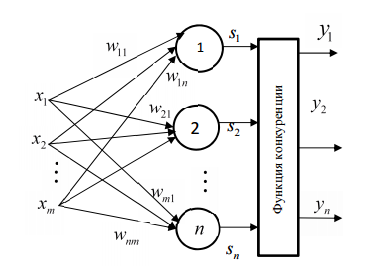
\includegraphics{network.png}
  \caption{Структура сети Кохонена}
  \label{img:network}
\end{figure}

\subsection{Слой Кохонена}

Слой Кохонена состоит из некоторого количества $n$ параллельно действующих линейных элементов. Все они имеют одинаковое число входов $m$ и получают на свои входы один и тот же вектор входных сигналов $x=(x_{1},...x_{m})$. На выходе $j$-го линейного элемента получаем сигнал 
\[
  y_{j}=w_{{j0}}+\sum _{{i=1}}^{m}w_{{ji}}x_{i},
\]
где:
\begin{itemize}
  \setlength\itemsep{0em}
  \item $w_{{ji}}$ — весовой коэффициент $i$-го входа $j$-го нейрона;
  \item $i$ — номер входа;
  \item $j$ — номер нейрона;
  \item $w_{{j0}}$ — пороговый коэффициент.
\end{itemize}

После прохождения слоя линейных элементов сигналы посылаются на обработку по правилу «победитель забирает всё»: среди выходных сигналов выполняется поиск максимального \(y_{j}\); его номер \(j_{{\max }}={{\rm {arg}}}\max _{{j}}\{y_{j}\}\). Окончательно, на выходе сигнал с номером \(j_{{\max }}\) равен единице, остальные — нулю. Если максимум одновременно достигается для нескольких \(j_{{\max }}\), то:
\begin{itemize}
  \setlength\itemsep{0em}
  \item либо принимают все соответствующие сигналы равными единице;
  \item либо равным единице принимают только первый сигнал в списке (по соглашению).
\end{itemize}

\subsection{Геометрическая интерпретация}

Большое распространение получили слои Кохонена, построенные следующим образом: каждому ($j$-му) нейрону сопоставляется точка $W_{j}=(w_{{j1}},...w_{{jm}})$ в $m$-мерном пространстве (пространстве сигналов). Для входного вектора $x=(x_{1},...x_{m})$ вычисляются его евклидовы расстояния $\rho _{j}(x)$ до точек $W_j$ и «ближайший получает всё» — тот нейрон, для которого это расстояние минимально, выдаёт единицу, остальные — нули. Следует заметить, что для сравнения расстояний достаточно вычислять линейную функцию сигнала:
\[
  \rho _{j}(x)^{2}=\|x-W_{j}\|^{2}=\|W_{j}\|^{2}-2\sum _{{i=1}}^{m}w_{{ji}}x_{i}+\|x\|^{2}
\]
(здесь $\|y\|$ — Евклидова длина вектора: $\|y\|^{2}=\sum _{i}y_{i}^{2}$). Последнее слагаемое $\|x\|^{2}$ одинаково для всех нейронов, поэтому для нахождения ближайшей точки оно не нужно. Задача сводится к поиску номера наибольшего из значений линейных функций:
\[
  j_{\max }={\rm {arg}}\max _{j}\left\{\sum _{i=1}^{m}w_{ji}x_{i}-{\frac {1}{2}}\|W_{j}\|^{2}\right\}
\]

Таким образом, координаты точки ${\displaystyle W_{j}=(w_{j1},...w_{jm})}$ совпадают с весами линейного нейрона слоя Кохонена (при этом значение порогового коэффициента ${\displaystyle w_{j0}=-\|W_{j}\|^{2}/2}$.

Если заданы точки $W_{j}=(w_{{j1}},...w_{{jm}})$, то $m$-мерное пространство разбивается на соответствующие многогранники Вороного-Дирихле $V_{j}$: многогранник $V_{j}$ состоит из точек, которые ближе к $W_j$, чем к другим $W_{k}$ ($k\neq j$).
\cite{wikipedia_network}

\subsection{Обучение сети Кохонена}

Сейчас мы рассмотрим, как при помощи сети Кохонена можно решить задачу классификации. Задача классификации отличается от задачи кластеризации тем, что нам заранее задано количество классов, на которые требуется разбить исходные данные.

Пусть у нас есть набор из $M$ исходных образов, который нужно классифицировать, т.е. разбить на K классов. Каждый образ будем описывать некоторым вектором
\[
  x^m = [x_1^m, x_2^m, ..., x_N^m],
\]
где $x_i^m$ суть действительные числа.

Обучать мы будем весовые коэффициенты
\[
  W^k = [w_1^k, w_2^k, ..., w_N^k],
\]
$k = 1, 2, ..., K$, где $K$ есть количество классов на которые мы разбиваем исходные образы. Заметим, что каждый вектор весов имеет такую же размерность, как и входные вектора.

Также скажем, что количество шагов обучения заранее определено, пусть это будет $T$.

Итак, алгоритм обучения сети:
\begin{enumerate}
  \item Нормировка исходных векторов.
  \begin{itemize}
    \item Вычислим $Max_n=\max_m x^m_n$, $Min_n=\min_m x^m_n$.
    \item Введем обозначения \(a_n = \dfrac1{Max_n-Min_n}, \; b_n=\dfrac{-Min_n}{Max_n-Min_n}\).
    \item Нормируем вектора $x^m_n=a_n x^m_n+b_n, \; n=1,...,N$.
  \end{itemize}
  \item Инициализируем веса случайным образом значениями от $0$ до $1$.
  \item Инициализируем $t = 0$.
  \item Для каждого $X_m$: \\
  ищем ближайший вектор $W_k$ и для найденного вектора $W_k$ корректируем компоненты:
  \[
    w^k_n=w^k_n+a(t)(x^m_n-w^k_n),  
  \]
  где $a(t) > 0$ - шаг обучения, убывающая функция.
  \item Если $t < T$, увеличиваем $t$ на 1, выполняем шаг 4
\end{enumerate}

Теперь наша сеть обучена, и мы можем приступать её к использованию.

Теперь любой вектор $X$ нужно нормировать и найти ближайший вектор $W_k$, где номер $k$ и будет номером класса. Поскольку мы инициализировали веса случайным образом, то собственно номера классов роли не играют, важно лишь группировка образов по классам.

Если к весам $W_k$ применить процедуру обратную к нормировке, то коэффициенты весов для каждого класса укажут средние значения компонент для класса.\cite{kohonen_network_learning}

Теперь же, когда мы изучили более простой вариант, перейдём к самоорганизующейся карте Кохонена - методу, который позволяет производить уже кластерный анализ.

\section{Самоорганизующаяся карта Кохонена}

Самоорганизующуюся карта - это разновидность сети Кохонена, которая позволяет не только производить кластеризацию объектов, но и выполнять многомерную визуализацию ее результатов.

Отличие самоорганизующейся карты от обычной сети Кохонена заключается в количестве выходных нейронов: в сети Кохонена оно должно соответствовать количеству кластеров, а в карте – количеству сегментов, из которого она должна состоять, т.е. размеру карты. Чем больше число сегментов в карте, тем детальнее она представляет распределение объектов в пространстве признаков.

Число входных нейронов карты, как и сети Кохонена, должно быть равно числу признаков, по которым производится кластеризация.

\begin{figure}[H]
  \centering
  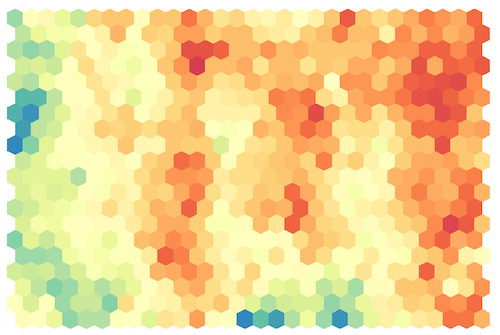
\includegraphics[width=0.7\textwidth]{every-cell-neuron.png}
  \caption{Примерная иллюстрация получаемой карты. Важно понимать, что, как правило, каждой ячейке соответствует один нейрон.}
  \label{every_cell_neuron}
\end{figure}

\subsection{Структура}

Самоорганизующаяся карта отличается от типичной нейронной сети и по своей архитектуре, и по алгоритмическим свойствам. Она состоит всего лишь из одного слоя вместо нескольких. Важным отличием алгоритма SOM является то, что в нем все нейроны (узлы, центры классов...) упорядочены в некоторую структуру(обычно двумерную сетку, см. Рис. \ref{img:structure}). При этом в ходе обучения модифицируется не только нейрон-победитель, но и его соседи, но в меньшей степени. За счет этого SOM можно считать одним из методов проецирования многомерного пространства в пространство с более низкой размерностью. При использовании этого алгоритма вектора, схожие в исходном пространстве, оказываются рядом и на полученной карте.\cite{basegroup}

\begin{figure}[h]
  \centering
  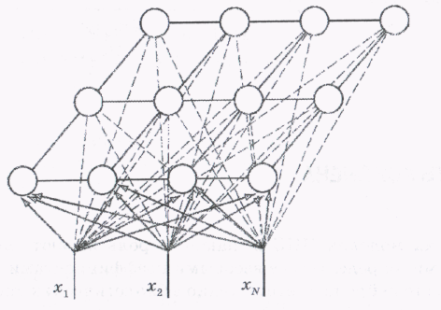
\includegraphics[width=0.5\textwidth]{structure.png}
  \caption{Структура сети, нейроны составляют двумерную сетку.}
  \label{img:structure}
\end{figure}

\subsection{Алгоритм обучения SOM}

Теперь рассмотрим алгоритм обучения SOM. По существу, он не сильно отличается от алгоритма обучения нейронной сети Кохонена. По ходу обучения мы также будем находить ближайший к вектору исходных данных $X_m$ вектор весов $W_k$ и изменять его, но изменения также будут затрагивать его соседей.

Пусть у нас есть набор из $M$ исходных образов, который нужно кластеризовать. Каждый образ будем описывать некоторым вектором
\[
  X^m = [x_1^m, x_2^m, ..., x_N^m],
\]
где $x_i^m$ суть действительные числа.

Обучать мы будем весовые коэффициенты
\[
  W^k = [w_1^k, w_2^k, ..., w_N^k],
\]
$k = 1, 2, ..., K$, где $K$ есть количество нейронов.

Количество шагов равно $\lambda$.

Алгоритм:
\begin{enumerate}
  \item инициализируем веса нейронов
  \item берём случайный вектор $X^t$ из множества входных данных, находим ближайший к нему нейрон (best matching unit, BMU), пусть $u$ - его индекс.
  \item изменяем веса нейронов по формуле:
  \[
    W^v(s + 1)=W^v(s)+\theta(u, v, s) \cdot \alpha(s) \cdot (X^t - W^v(s)),
  \]
  где:
  \begin{itemize}
    \setlength\itemsep{0em}
    \item $W^v(s)$ - веса нейрона $W_v$ на итерации $s$.
    \item $\theta(u, v, s)$ - расстояние между нейронами $W^u$ и $W^v$. Обычно используется один из двух вариантов: либо функция Гаусса, либо же расстояние до соседей равно 1, а до остальных нейронов оно приравнивается 0.
    \item $\alpha(s) > 0$ - шаг обучения, убывающая функция.
  \end{itemize}
  \item повторяем c шага 2, пока $s < \lambda$.\cite{algorithm}
\end{enumerate}

Отметим, что предложенный алгоритм не использует явно никакого критерия оптимизации. Хотя ясно, что, по крайней мере, будет уменьшаться среднее расстояние от каждой точки данных до ближайшего узла карты. Средний квадрат такого расстояния иногда используют для оценки точности карты.\cite{zinovyevbook}

После завершения обучения мы разбиваем нейроны на отдельные кластеры. И теперь мы можем кластеризовать исходные данные, занося их кластеры, которым принадлежат ближайшие к ним нейроны. Пример разбиения нейронов на кластеры вы можете видеть на Рис. \ref{img:congress}

\begin{figure}[H]
  \centering
  \def\svgwidth{\textwidth}
  \input{../img/Somtraining.pdf_tex}
  \caption{Иллюстрация того, как веса нейронов в процессе обучения постепенно приближаются к исходным данным.}
  \label{somtraining}
\end{figure}

\subsection{Методы представления}

После того, как самоорганизующейся карта обучена, нам необходимо как-то взглянуть на получившийся результат. Существует несколько стандартных способов это сделать, и сейчас мы их рассмотрим.

\subsubsection{U-matrix}

Унифицированная матрица расстояний(U-матрица, U-matrix, unified distance matrix) - это одно из представлений самоорганизующейся карты. Она визуализирует расстояния между нейронами. Расстояние между соседними нейронами вычисляется и представляется в виде различной окраски между соседними узлами. Темная окраска между нейронами соответствует большому расстоянию и, следовательно, разрыву между значениями во входном пространстве. Светлая окраска между нейронами означает, что векторы находятся близко друг к другу во входном пространстве. Светлые области можно рассматривать как кластеры, а темные - как разделители кластеров. Это может быть полезным представлением, когда вы пытаетесь найти кластеры во входных данных, не имея никакой априорной информации о них.\cite{u_matrix} Пример U-matrix приведён на Рис. \ref{u-matrix} Также существует трёхмерное расширение U-matrix - U-array (см. Рис. \ref{u-array-rec}) 

\begin{minipage}{0.5\textwidth}
\begin{figure}[H]
  \centering
  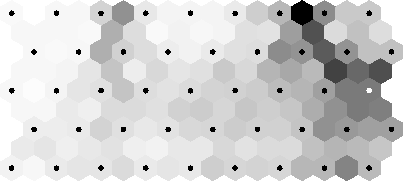
\includegraphics[width=0.8\textwidth]{u-matrix.png}
  \caption{Пример U-matrix. Чёрные точки обозначают нейроны, чем больше расстояние между соседними нейронами, тем темнее ячейки, находящиеся между ними.}
  \label{u-matrix}
\end{figure}
\end{minipage}
\begin{minipage}{0.5\textwidth}
  \begin{figure}[H]
    \centering
    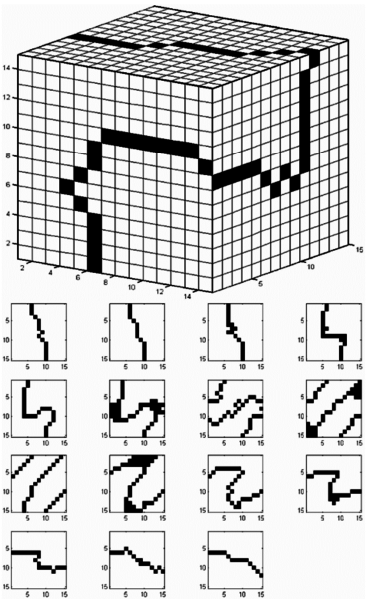
\includegraphics[width=0.5\textwidth]{u-array-rec.png}
    \caption{U-array - трёхмерная U-matrix}
    \label{u-array-rec}
  \end{figure}
\end{minipage}

\subsubsection{Карта входов нейронов}

Карта входов нейронов строится для каждого входа ($x_i$), где нейроны раскрашиваются в соответствии с весом $w_i$, соответствующим этому входу. Пример можно увидеть на рис. \ref{img:congress}, где все карты, кроме первых трёх, являются картами входов.

\subsubsection{Карта выходов нейронов}

На карту выходов нейронов проецируется взаимное расположение исследуемых входных данных. Примером служит правая нижняя карта на Рис. \ref{img:fisher}

\subsubsection{Специальные карты}

Это карта кластеров, матрица расстояний(U-matrix), матрица плотности попадания и другие карты, которые характеризуют кластеры, полученные в результате обучения сети Кохонена. Примером служат первые две карты из рис. \ref{img:congress}

Важно понимать, что между всеми рассмотренными картами существует взаимосвязь - все они являются разными раскрасками одних и тех же нейронов. Каждый пример из обучающей выборки имеет одно и то же расположение на всех картах.\cite{intuit}

\subsection{Вычисление расстояний в U-matrix}

В данном пункте мы углубимся в вопрос вычисления расстояний для построения U-matrix. В этом нам поможет работа \cite{distance}, в которой приведены формулы и соответствующие пояснения.

Унифицированная матрица для двумерных карт (U-matrix) имеет размерность $(2n-1)$x$(2m-1)$, где $n$-число нейронов по оси $x$, $m$ – число нейронов по оси $y$. U-matrix включает в себя следующие расстояния между нейронами: $dx(x,y)$, $dy(x,y)$ и $dxy(x,y)$.

\begin{figure}[H]
  \centering
  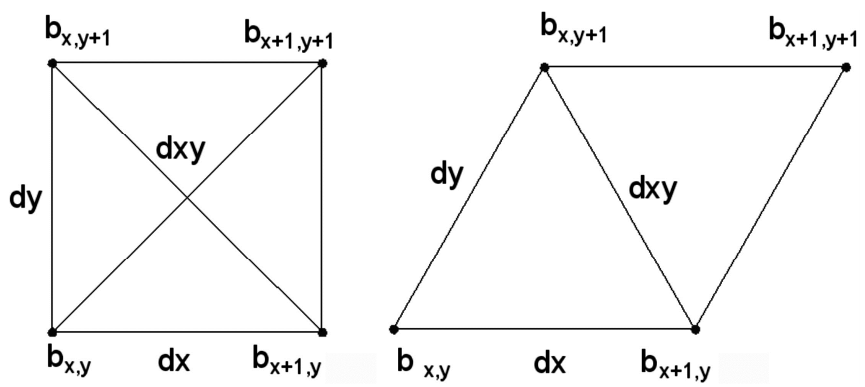
\includegraphics[width=0.6\textwidth]{u-matrix-distance.png}
  \caption{Обозначения для прямоугольной и гексогональной решёток}
  \label{img:u-matrix-distance}
\end{figure}

Для прямоугольной и гексогональной матрицы $dx(x, y)$ и $dy(x, y)$ вычисляются одинаково:

$$\begin{aligned}
  &d x(x, y)=\left\|b_{x, y}-b_{x+1, y}\right\|=\sqrt{\sum_{i}\left(w_{i_{x, y}}-w_{i_{x+1} y+1}\right)^{2}}\\
  &d y(x, y)=\left\|b_{x, y}-b_{x, y+1}\right\|=\sqrt{\sum_{i}\left(w_{i_{x, y}}-w_{i_{x, y+1}}\right)^{2}}
\end{aligned}$$

А вот $dxy(x, y)$ отличается. Например, для прямоугольной:
$$\begin{aligned}
  &d x y(x, y)=\frac{1}{2}\left(\frac{\left\|b_{x, y}-b_{x+1, y+1}\right\|}{\sqrt{2}}+\frac{\left\|b_{x, y+1}-b_{x+1, y}\right\|}{\sqrt{2}}\right)=\\
  &=\frac{1}{2 \sqrt{2}}[\sqrt{\sum_{i}\left(w_{i_{x y}}-w_{i_{x+1}, y_{+1}}\right)^{2}}+\sqrt{\sum_{i}\left(w_{i_{x y+1}}-w_{i_{x+1, y}}\right)^{2}}]
  \end{aligned}$$

и для гексогональной:

$$d x y(x, y)=\left\|b_{x, y+1}-b_{x+1, y}\right\|=\sqrt{\sum_{i}\left(w_{i_{x y}+1}-w_{i_{x+1, y}}\right)^{2}}$$

\subsubsection{Вычисление расстояний в U-array}

U-array является расширением U-matrix для трехмерных карт. Этот массив будет иметь размерность $(2n-1)$x$(2m-1)$x$(2p-1)$, где $p$ - число нейронов по оси $z$. U-array включает в себя дополнительные дистанции: $dz(x,y,z)$, $dxz(x,y,z)$, $dyz(x,y,z)$ и $dxyz(x,y,z)$. Расстояние $dz(x,y,z)$ рассчитывается аналогично расстояниям $dx(x,y)$ и $dy(x,y)$. Расстояния $dxz(x,y,z)$ и $dyz(x,y,z)$ рассчитываются таким же способом, как и расстояние $dxy(x,y)$.

\begin{figure}[H]
  \centering
  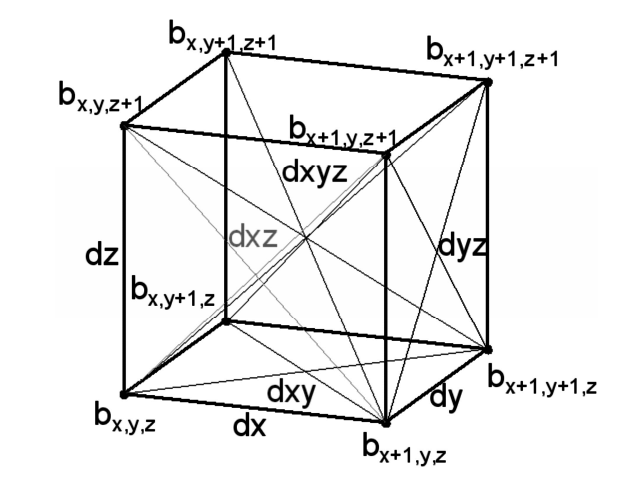
\includegraphics[width=0.5\textwidth]{u-array-rec-distance.png}
  \caption{Обозначение расстояний U-array для прямоугольной решётки}
  \label{u-array-rec-distance}
\end{figure}

Расстояние $dxyz(x,y,z)$ на прямоугольной решётке можно рассчитывать по следующей формуле:

$$\begin{aligned}
  &d x y z(x, y, z)=\frac{1}{4}\left(\frac{\left\|b_{x, y, z}-b_{x+1, y+1, z+1}\right\|}{\sqrt{3}}+\right.\\
  &+\frac{\left\|b_{x+1, y, z}-b_{x, y+1, z+1}\right\|}{\sqrt{3}}+\frac{\left\|b_{x+1, y+1, z}-b_{x, y, z+1}\right\|}{\sqrt{3}}+\\
  &+\frac{\left\|b_{x, y+1, z}-b_{x+1, y, z+1}\right\|}{\sqrt{3}}=\\
  &=\frac{1}{4 \sqrt{3}}\left[ \sqrt{\sum_{i}\left(w_{i_{x, y, z}}-w_{i_{x+1, y+1, z+1}}\right)^{2}}+\right.\\
  &+\sqrt{\sum_{i}\left(w_{i_{x+1, y, z}}-w_{i_{x, y+1, z+1}}\right)^{2}}+\\
  &+\sqrt{\sum_{i}\left(w_{i_{x+1, y+1, z}}-w_{i_{x, y, z+1}}\right)^{2}}+\\
  &\left.+\sqrt{\sum_{i}\left(w_{i_{x, y+1, z}}-w_{i_{x+1, y, z+1}}\right)^{2}} \right]
  \end{aligned}$$

Для вычисления расстояний на гексогональной карте требуется уже несколько больших групп формул, поэтому для тех, кто хочет разобраться в этом вопросе, снова привожу ссылку на статью \cite{distance} и предлагаю ознакомиться самостоятельно.

\section{Примеры использования}

Рассмотрим несколько примеров использования карт.

\begin{enumerate}
  \item Пример из области политики. Здесь сеть обучена на наборе данных о Конгрессе США.
  \begin{figure}[H]
    \centering
    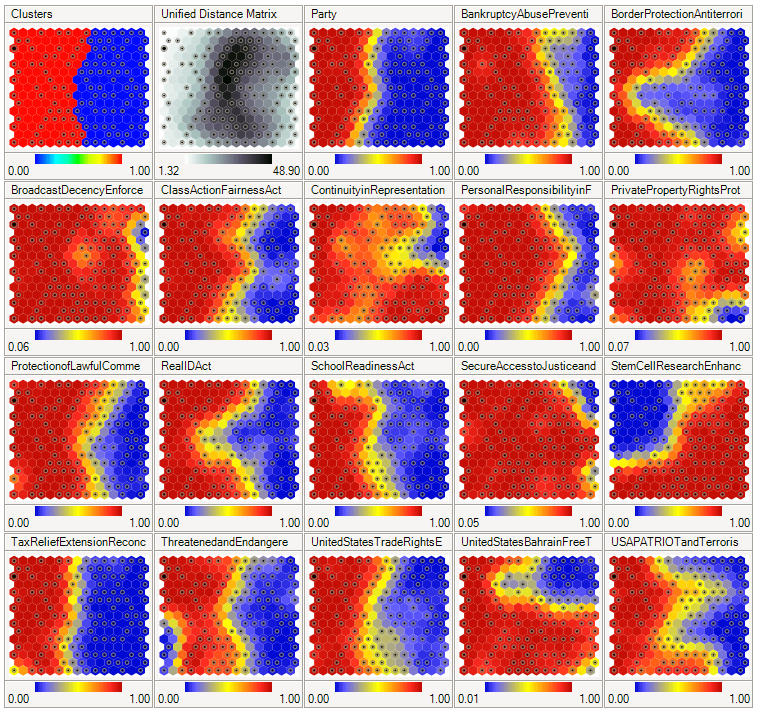
\includegraphics[width=0.5\textwidth]{congress.png}
    \caption{Самоорганизующаяся карта, показывающая схему голосования в Конгрессе США. Исходные данные представляли собой таблицу со строкой для каждого члена Конгресса и столбцами для определенных голосов, содержащими голос каждого члена " да " / " нет " / "воздержался". Алгоритм SOM расположил эти элементы в двумерной сетке, расположив подобные элементы ближе друг к другу. Первый график показывает группировку, когда данные разделены на два кластера. Второй график показывает среднее расстояние до соседей: большие расстояния темнее. Третий график предсказывает членство в Республиканской (красной) или Демократической (синей) партии. Остальные графики являются картами по одному из входов(карта входов нейронов): красный цвет означает предсказанный голос "да" по этому законопроекту, синий - голос "нет".\cite{wikipedia_map_en}}
    \label{img:congress}
  \end{figure}

  \item Здесь сеть обучена на наборе данных "Ирисы Фишера"\cite{fishers_irises}.
  \begin{figure}[H]
    \centering
    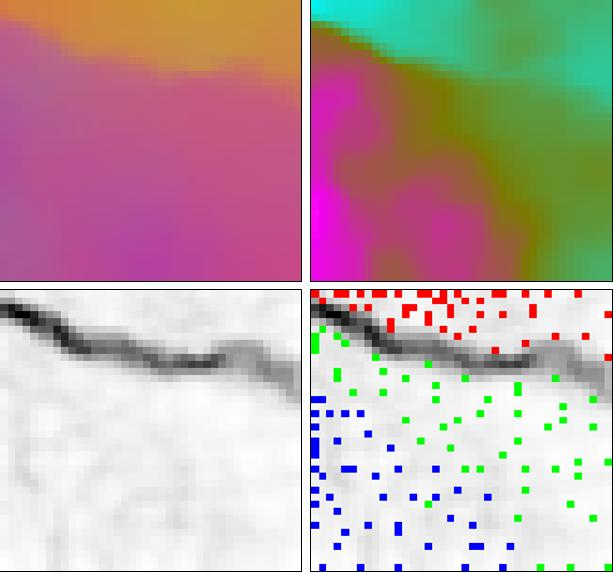
\includegraphics[width=0.5\textwidth]{som_fisher.jpeg}
    \caption{
      Самоорганизующаяся карта, натренированная на наборе данных "Ирисы Фишера"\cite{fishers_irises}. Вверху слева: цветное изображение, образованное первыми тремя измерениями четырехмерных весовых векторов нейронов SOM. Вверху справа: псевдоцветное изображение величины векторов веса SOM. Внизу слева: U-Матрица (Евклидово расстояние между весовыми векторами соседних ячеек). Внизу справа: карта выходов нейронов, наложение точек данных (красный: I. setosa, зеленый: I. versicolor и синий: I. virginica) на U-матрицу, основанную на минимальном евклидовом расстоянии между векторами данных и весовыми векторами SOM.
    }
    \label{img:fisher}
  \end{figure}

  \item В данной \href{https://habr.com/ru/post/334810/}{статье} автор показывает, как в Python сгенерировать набор данных, а потом обучить на нём сеть Кохонена.

  В ней он сначала генерирует множество трёхмерных векторов(цвета в пространстве RGB) и обучает на нём сеть, созданную в TensorFlow. Результаты приведены ниже.\cite{habr}

  \begin{figure}[H]
    \centering
    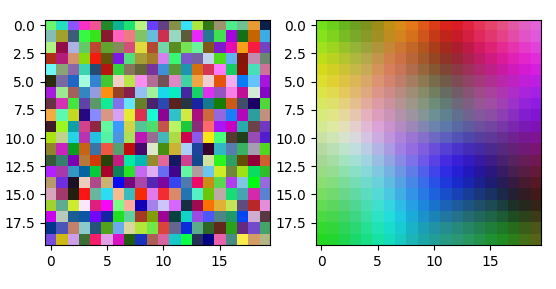
\includegraphics[width=\textwidth]{habr-20.png}
    \caption{Карта весов в начале обучения (слева) и в конце обучения (справа) для 20 нейронов.}
  \end{figure}

  \begin{figure}[H]
    \centering
    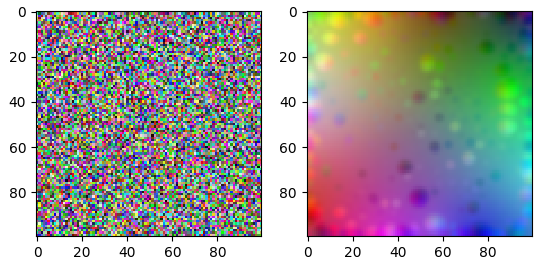
\includegraphics[width=\textwidth]{habr-100.png}
    \caption{Карта весов для сети 100x100 нейронов, после 350тыс. итераций обучения.}
  \end{figure}
\end{enumerate}

\section{Вопросы}

\begin{enumerate}
  \item слой Кохонена
  \item геометрическая интерпретация
  \item структура самоорганизующихся карт
  \item алгоритм обучения SOM
  \item методы представления
\end{enumerate}

\begin{thebibliography}{9}
  \bibitem{intro1}
    \url{https://ami.nstu.ru/~vms/lecture/data_mining/kurs_klaster.htm}

  \bibitem{clustering}
    \href{https://neerc.ifmo.ru/wiki/index.php?title=\%D0\%9A\%D0\%BB\%D0\%B0\%D1\%81\%D1\%82\%D0\%B5\%D1\%80\%D0\%B8\%D0\%B7\%D0\%B0\%D1\%86\%D0\%B8\%D1\%8F}
    {https://neerc.ifmo.ru/wiki/index.php?title=Кластеризация}

  \bibitem{intro2}
    \url{https://docplayer.ru/57111584-Soderzhanie-vvedenie-zadacha-klasterizacii-dannyh-ponyatie-klasterizacii-postanovka-zadachi-klasterizacii.html}

  \bibitem{scholarpedia}
    Teuvo Kohonen and Timo Honkela (2007)
    \href{http://www.scholarpedia.org/article/Kohonen_network}{Kohonen network}.
    \href{http://www.scholarpedia.org/}{Scholarpedia},
    2(1):1568.

  \bibitem{wikipedia_network}
    \href{https://ru.wikipedia.org/wiki/\%D0\%9D\%D0\%B5\%D0\%B9\%D1\%80\%D0\%BE\%D0\%BD\%D0\%BD\%D0\%B0\%D1\%8F\_\%D1\%81\%D0\%B5\%D1\%82\%D1\%8C\_\%D0\%9A\%D0\%BE\%D1\%85\%D0\%BE\%D0\%BD\%D0\%B5\%D0\%BD\%D0\%B0}
    {https://ru.wikipedia.org/wiki/Нейронная\_сеть\_Кохонена}

  \bibitem{wikipedia_map_ru}
    \href{https://ru.wikipedia.org/wiki/\%D0\%A1\%D0\%B0\%D0\%BC\%D0\%BE\%D0\%BE\%D1\%80\%D0\%B3\%D0\%B0\%D0\%BD\%D0\%B8\%D0\%B7\%D1\%83\%D1\%8E\%D1\%89\%D0\%B0\%D1\%8F\%D1\%81\%D1\%8F_\%D0\%BA\%D0\%B0\%D1\%80\%D1\%82\%D0\%B0_\%D0\%9A\%D0\%BE\%D1\%85\%D0\%BE\%D0\%BD\%D0\%B5\%D0\%BD\%D0\%B0}
    {https://ru.wikipedia.org/wiki/Самоорганизующаяся\_карта\_Кохонена}

  \bibitem{wikipedia_map_en}
    \href{https://en.wikipedia.org/wiki/Self-organizing\_map}{https://en.wikipedia.org/wiki/Self-organizing\_map}

  \bibitem{algorithm}
    \href{https://en.wikipedia.org/wiki/Self-organizing\_map\#Algorithm}
    {https://en.wikipedia.org/wiki/Self-organizing\_map\#Algorithm}

  \bibitem{basegroup}
    \href{https://basegroup.ru/community/articles/som}{https://basegroup.ru/community/articles/som}

  \bibitem{intuit}
    \href{https://www.intuit.ru/studies/courses/6/6/lecture/180?page=3}{https://www.intuit.ru/studies/courses/6/6/lecture/180?page=3}
  
  \bibitem{u_matrix}
    \url{https://users.ics.aalto.fi/jhollmen/dippa/node24.html}

  \bibitem{kohonen_network_learning}
    \url{http://ai.lector.ru/?go=lection04}
  
  \bibitem{fishers_irises}
    \href{https://ru.wikipedia.org/wiki/\%D0\%98\%D1\%80\%D0\%B8\%D1\%81\%D1\%8B_\%D0\%A4\%D0\%B8\%D1\%88\%D0\%B5\%D1\%80\%D0\%B0}
         {https://ru.wikipedia.org/wiki/Ирисы\_Фишера}

  \bibitem{zinovyevbook}
    \url{http://pca.narod.ru/ZinovyevBook.pdf}
  
  \bibitem{habr}
    \url{https://habr.com/ru/post/334810/}

  \bibitem{distance}
    \url{http://www.dspa.ru/articles/year2015/jour15_2/art15_2_4.pdf}
\end{thebibliography}

\end{document}